
\subsection{Product perspective}
\begin{minipage}{\textwidth}
The following Class Diagrams represent the three services and the domain model where they work.
White class are dedicated to perform Data4Help service, the other two applications are listed below.
\begin{center}
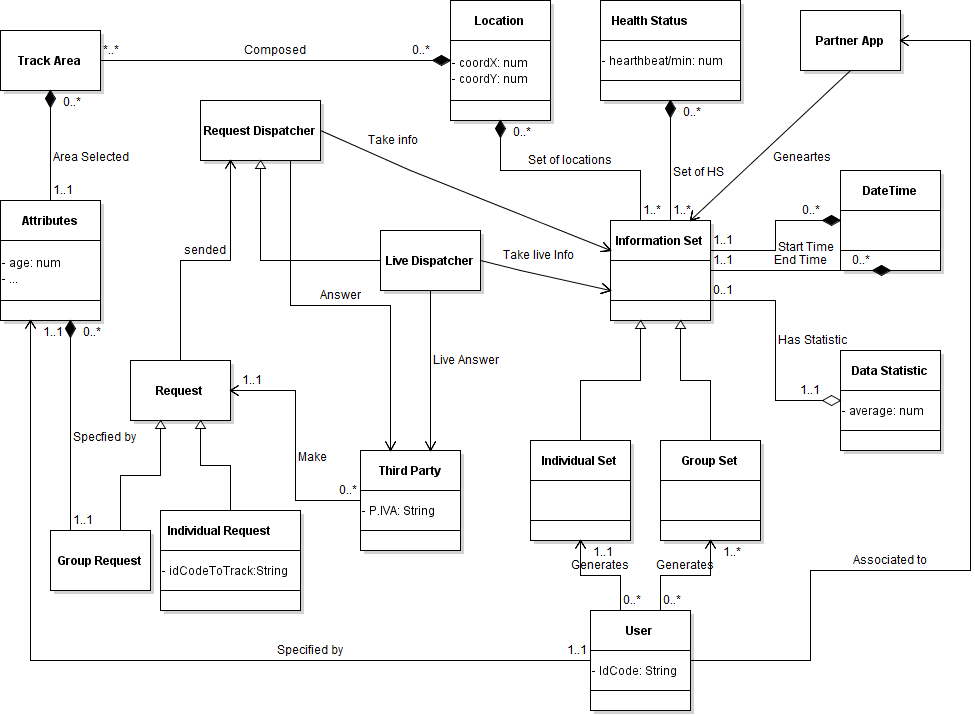
\includegraphics[scale=0.45]{Images/Class_Data4Help.png}
\end{center}
\bigbreak
{\color{Salmon} Red classes} are dedicated to {\color{Salmon} AutomatedSOS} application, supported by Data4Help service (white ones).
\begin{center}
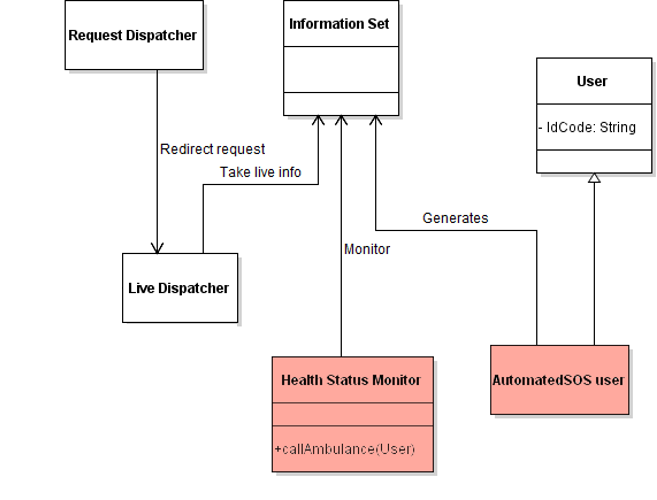
\includegraphics[scale=0.55]{Images/Class_AutoSOS.png}
\end{center}
\end{minipage}
\clearpage

\begin{minipage}{\textwidth}
{\color{LimeGreen} Green classes} are dedicated to {\color{LimeGreen} Track4Run} application, supported by Data4Help service (white ones).
\begin{center}
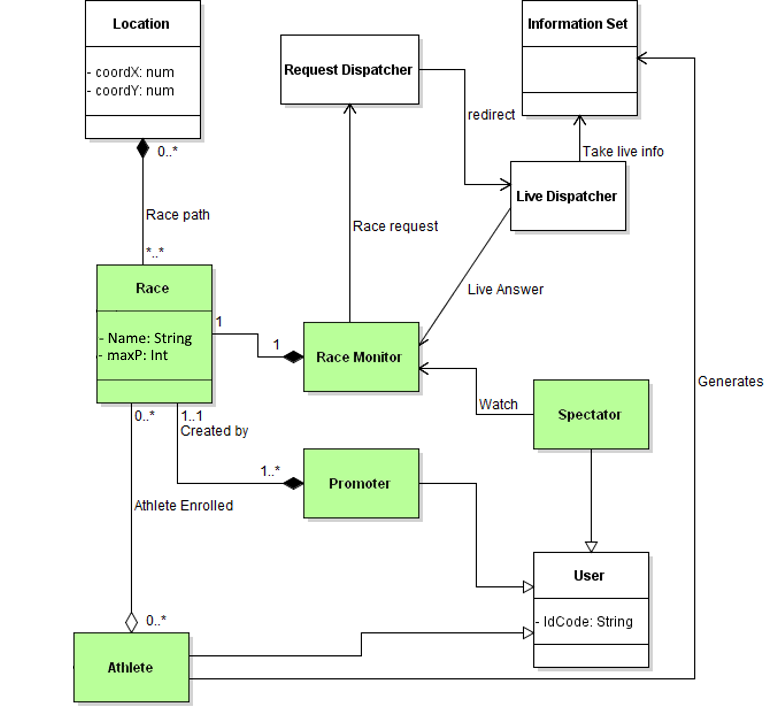
\includegraphics[scale=0.7]{Images/Class_Track4Run.png}
\\[1 cm]
\end{center}
The following State Chart represents the behaviour of a Data Request Object.
\begin{center}
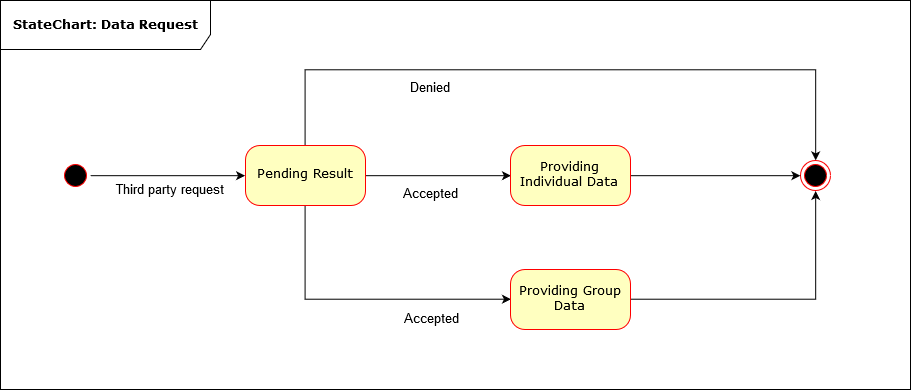
\includegraphics[scale=0.5]{Images/StateChart.png}
\end{center}
\end{minipage}

\subsection{Product functions}
The systems-to-be under analysis have to offer several functions. Below, the main functions provided by each system are more precisely specified, considering all the aspects emerged from the previous list of goals.
\subsubsection{Data4Help - Providing data to third parties }
This is the core function that Data4Help has to ensure. After collecting users position and health status information from external partner applications, Data4Help provides these data to the third party interested in having them. Data4Help provides data on demand sending to the third party all the available data about an individual (or a group of individual) collected so far. So the third party is provided with all the data about a user collected until now. In addition, Data4Help offers a providing data service in real time, allowing the third party to subscribe to new data and to receive them as soon as they are produced. TrackMe in order to offer a complete solution to third parties send them also statistics about data.

\subsubsection{AutomatedSOS - Sending ambulance request in critical situation}
AutomatedSOS monitors the health status of the subscribed customers and, when such parameters are below certain threshold, sends to the location of the customer an ambulance, guarantying a reaction time of less than 5 seconds from the time parameters are below the threshold.
\bigbreak
\noindent
Therefore, the main function offered by AutomatedSOS is sending an ambulance request, with the relative user position, to the nearest hospital to the user. In order to optimize the times, the ambulance request contains all the data about the user health status. Providing these information, when rescue arrives, it can immediately act accordingly to the received data. AutomatedSOS retrives data directly from the user's smartwatch and send them to Data4Help. In order to keep under control the user's health status AutomatedSOS performs monitoring using these retrieved data and other hystorical data got from Data4Help, the latter are used to have a profile of the user's health status.
\subsubsection{Track4Run - Run management}
Track4Run offers three different functionality for its users, which can be all grouped under the 'run management' function. A user can be a promoter, in this case the user can create the event run , which will be visible to every other users. Once created a run, the promoter can define the path in an interactive way, that is by drawing the path directly on a map. Track4Run allows the promoter to set other additional information, like the start time or an overall description of the run. Finally, the promoter can invite to the run all the participants. Every run can be enrolled by everyone, so the scope of inviting a person is just to promote the run and to facilitate the enrollment process.
\bigbreak
\noindent
The athletes have to be user too. Once received a run request, the athlete can enroll the run or reject it. In the first case, Track4Run tracks in real time the participant position for all the run through a smartwatch. 
\bigbreak
\noindent
A user can also be a simple spectator and see on a map the position of all runners during the run. A spectator is also provided with the main information about the participants and with live time laps.

\subsection{User characteristics}
\begin{enumerate}
\item Third party: Company interested in retrieving useful data from TrackMe's users. Usually, this information can be relevant for marketing strategy.

\item User: Individual whose data are acquired from TrackMe through Data4Help service and are provided to third parties. AutomatedSOS is a service thought for elderly people, while Track4Run is a service thought for athletes, promoters and spectators of runs. User's privacy is protected by each service.

\end{enumerate}

\subsection{Assumptions, dependencies and constraints}
In the specification document certain parts are not specified and a bit ambiguous. So we decided to make the following assumptions.

\subsubsection{Text Assumptions}
\begin{enumerate}

\item[•] {\Large Data4Help}
	\begin{enumerate}
	\item User's data are collected from partner applications or from the other two TrackMe applications installed on user's devices.
	\item Partner applications can be all the sport assistant apps, GPS assistant apps or all the other applications that can retrieve location and health status of individual for such reason.
	\item All the partner applications require to submit user credentials. 
	\item When the partner application is installed and credentials are submitted,
	the user is required to accept privacy policy, composed in two parts:
		\begin{enumerate}
		\item The first, mandatory, user accept to be tracked in group mode.
		\item The second, optional, user accept to be tracked in single mode.
		\end{enumerate}
	\item Individual monitoring requests are not accepted or denied one by one by the specific user. If the user agreed on the treatment of his data as information of an individual (second part of privacy policy) all individual request by third parties are automatically accepted.	
	\item Data are collected from partner application only when they are active on user's device.
	\item Only third parties that are registered to Data4Help can request the monitoring service.
	\item Groups are characterized by its members' attributes (age, gender, city, …).
	\item Health status parameters that can be acquired are all the ones supported by a standard smartwatch as: Heart Rate, Blood Pressure, Pedometer, Calories Calculation.
	\item The answers to both Individual Requests and Group Requests contain also some statistics other than raw data.
	\item Live acquisition request expires after one month from the moment that is formulated.
	\end{enumerate}
	
\item[•] {\Large AutomatedSOS}
	\begin{enumerate}
	\item AutomatedSOS exploit only smartwatches devices to retrieve all the information needed.
	\item AutomatedSOS is an application that needs to be installed into the user's device.
	\item All data retrieved by AutomatedSOS are sent to Data4Help.
	\item In any case, data retrieved by AutomatedSOS won't be sent to third parties if they perform an individual request. Thus TrackMe doesn't offer additional services for third parties through AutomatedSOS.
	\item In order to keep under systematic review the user's health status and have a broad view of it, some historical information about the user are received by Data4Help's Database.
    \item This service can be used only by elderly people (70+) or by who really need it, in order to avoid useless waste of resources.
    \item User can see all personal information that have been sent to the Data4Help service. 
	\end{enumerate}
	
\item[•] {\Large Track4Run}
	\begin{enumerate}
	\item During the registration to the application the user is asked to accept or deny the treatment of his data by  Data4Help service.
	\item The application has three functions: 
	\begin{enumerate}
	\item Promoter: allow the user to manage a run.  
	\item Athlete: allow the user to participate to a run. In order to be an athlete the request of data treatment by the Data4Help service need to be accepted.
	\item Spectator: Allow the user to watch in real time the positions of all the athletes in a given run.
	\end{enumerate}
	\item All run events are seen as public runs, so every user can enroll to future runs.
	\item Any user can organize an event and also invite other users to enroll to the run.
    \item All the events can be spectated by users.
    \item All users invited to a run can accept or discard the request.
    \item Race path are always composed by citizen routes (never in private circuits or stadiums)
    \end{enumerate}
\end{enumerate}

\subsubsection{Domain Assumptions}
\begin{enumerate}

\item[•] {\Large Data4Help}
	\begin{enumerate}
	\item [D.1] User's information are collected from partner applications or from the other two TrackMe applications installed on users' devices.
	\item [D.2] All the partner applications require to submit user credentials.
	\item [D.3] The identification (fiscal code, social security number) and the secondary data (attributes) given by the individual during the registration are correct.
    \item [D.4] Devices used to monitor individuals always report correct values.
    \item [D.5] Partner application always report correct values to Data4Help.
	\item [D.6] In order to perform an individual request, third parties has to know the user's fiscal code or security number.
	\item [D.7] Security number and fiscal code are not information given to third parties by Data4Help.
	\end{enumerate}
	
\item[•] {\Large AutomatedSOS}
	\begin{enumerate}
	\item [D.4] Devices used to monitor individuals always report correct values.
	\item [D.9] The user always dresses a smartwatch on which AutomatedSOS is installed and running.    
	\item [D.10] The first aid system is always up and ready to receive messages from AutomatedSOS.
    \item [D.11] The ambulance successfully reach the location of the individual.
    \item [D.12] The ambulance always get to the location in the minimum amount of time.
    
	\end{enumerate}
	
\item[•] {\Large Track4Run}
	\begin{enumerate}
	\item [D.4] Devices used to monitor individuals always report correct values.
	\item [D.13] During a run athletes always wear a smartwatch on which Track4Run is installed.
	\item [D.14] The path defined by the organizer actually exist.
    \item [D.16] If an athlete enroll to a run then athlete also participates to the run.
    \item [D.17] All athletes have their tracking devices with them and the application is enabled for the entire duration of the run.
    \item [D.18] Athletes never go out of the defined path.
	\end{enumerate}
\end{enumerate}